\qquad A análise de complexidade do Bubble Sort, considerando as
diferentes situações de entrada (crescente, decrescente e
randômica), foi realizada manuscrita, com a devida justificativa,
conforme exigido pelo enunciado do trabalho. A digitalização do
material manuscrito deve ser inserida a seguir, substituindo a
imagem de exemplo abaixo.

\begin{figure}[htbp]
    \centering
    % Substitua o arquivo abaixo pela digitalizacao da analise de complexidade manuscrita
    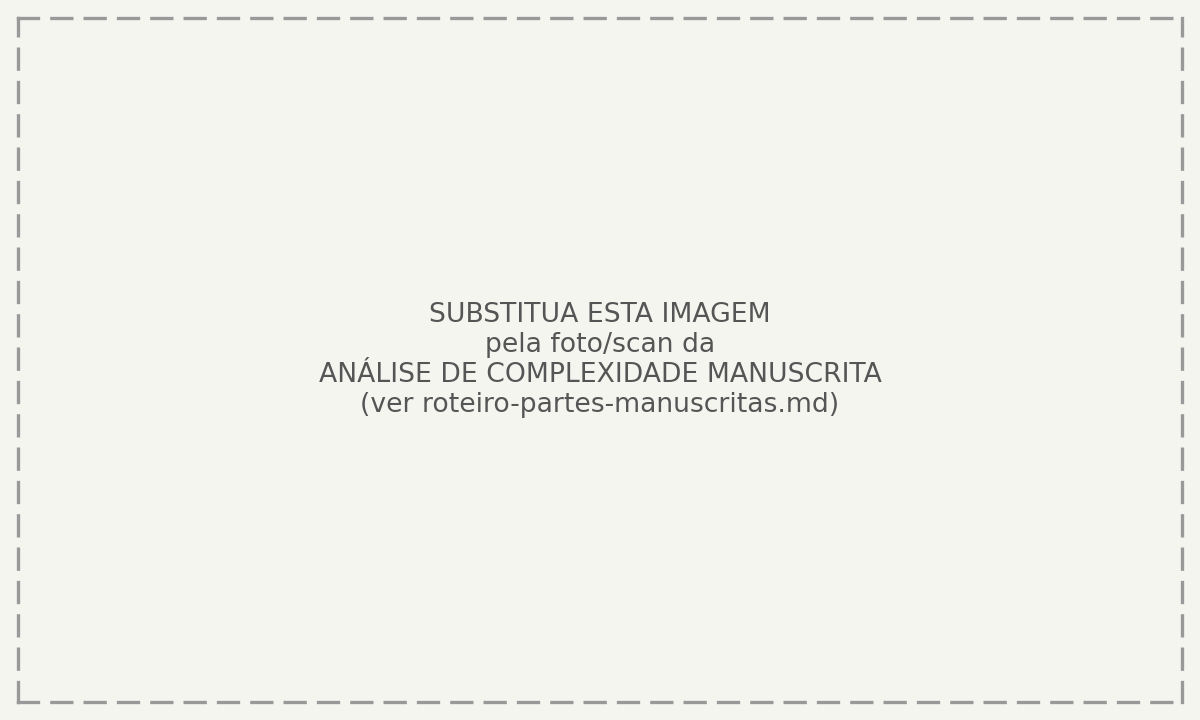
\includegraphics[width=14cm]{Imagens/Bubble Sort/analise_complexidade.png}
    \caption{Análise de complexidade manuscrita do algoritmo Bubble Sort}
    \label{fig:analise_complexidade_bubble}
\end{figure}

\qquad Os resultados experimentais apresentados na próxima seção deste
capítulo são compatíveis com essa análise teórica: desempenho linear
no melhor caso (entrada crescente, graças à parada antecipada quando
nenhuma troca ocorre em uma passada) e desempenho quadrático no caso
médio e no pior caso (entradas randômica e decrescente). Vale destacar
que, apesar de Insertion Sort e Bubble Sort compartilharem a mesma
ordem de grandeza no pior caso, o Bubble Sort tende a ser mais lento
na prática, pois cada troca custa três atribuições, contra apenas uma
atribuição por deslocamento no Insertion Sort — o que também é
confirmado pelos tempos medidos.
